\documentclass[11pt, fleqn]{article}

\usepackage{amsmath}
\usepackage{amsfonts}
\usepackage[margin=1in]{geometry} % To set the margin widths
\usepackage{graphicx}
\usepackage{listings}
\usepackage{multirow}
\usepackage{tabularx}
\usepackage{varioref}
\usepackage{cleveref}
\usepackage{siunitx}
\usepackage{subcaption}
\usepackage{titlesec}
\usepackage{bm}

\lstset{
  language=R,
  literate = {<-}{{$\gets$}}1 {~}{{$\sim$}}1
}

\sisetup{output-exponent-marker=\textsc{e}}

\titleformat{\section}[block]{\bfseries}{\thesection}{1em}{}

\setlength{\parskip}{12pt} % Sets a blank line in between paragraphs
\setlength\parindent{0pt} % Sets the indent for each paragraph to zero

\begin{document}

\title{Big Data: Homework 4}
\author{Will Clark \& Matthew DeLio \\ 41201-01}
\date{\today}
\maketitle

\section{Network Connectivity Transformation}

Network connectivity (which we are calling \texttt{degree}) is measured by the number of edges for each node in a network. In this context, \texttt{degree} measures the number of relationships that a household in our population has. We observe in Figure~\ref{fig:degrees} that \texttt{degree} is distributed logarithmically.

\begin{figure}[!htb]
  \centering
  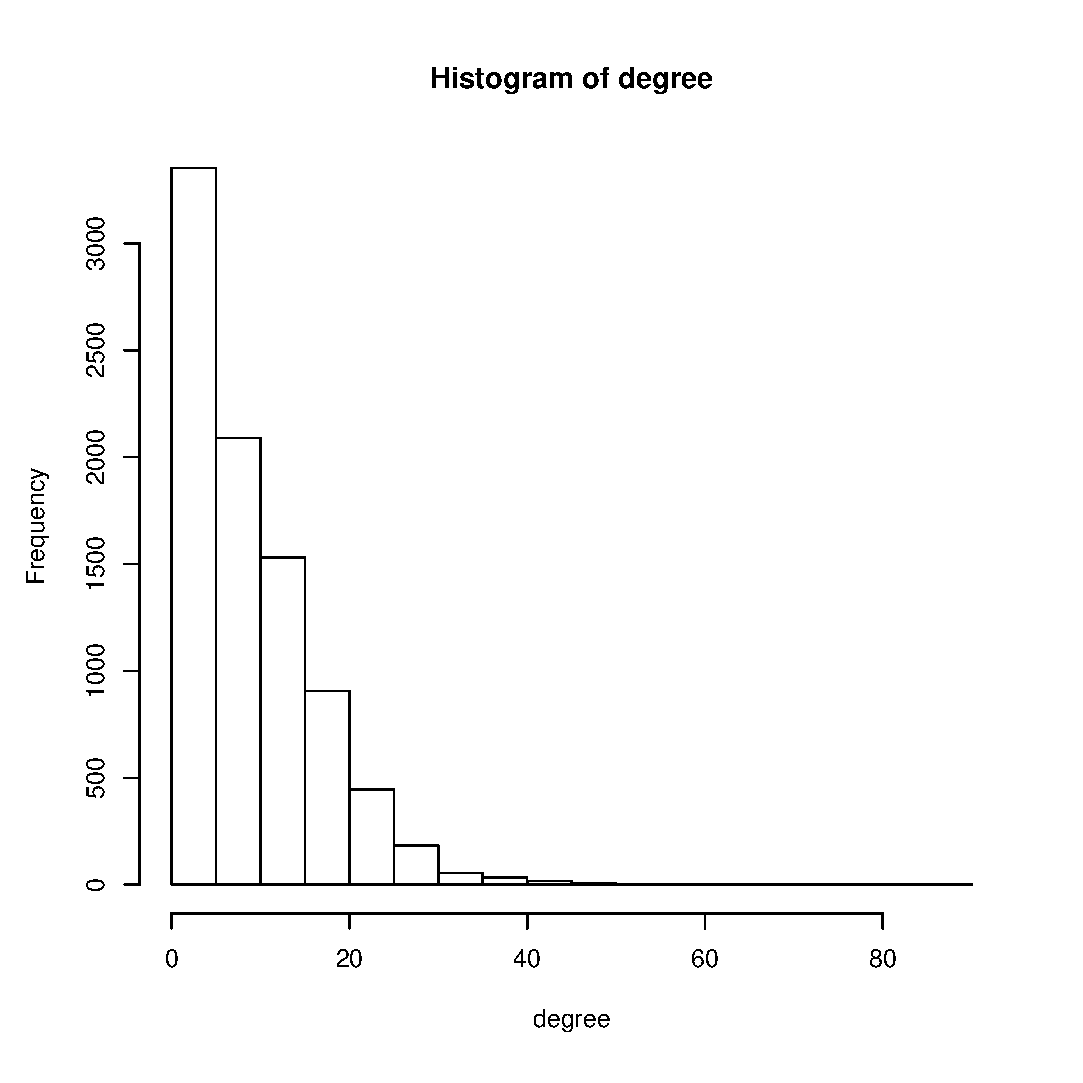
\includegraphics[scale=.5]{degrees.eps}
  \caption{Distribution of \texttt{degree}}
  \label{fig:degrees}
\end{figure}

\section{Predicting Network Connectivity from Controls}

\section{Effect of Network Connectivity on Loan Propensity}

\section{Naive Estimation of Loan Propensity}

\section{Bootstrapping Uncertainty}

\section{Experimental Design}

\end{document}
